\documentclass[xcolor=x11names,table]{beamer}
\usetheme{Bergen}  % CambridgeUS theme
\usecolortheme{spruce}
\usepackage{float}  % perfect fit graphic with command [H]
%\usepackage{tabularx}  % alternate to tabular to use X to wrap column data properly
%\usetheme{Antibes}
\usepackage{hyperref}

%package for timeline
\usepackage[utf8]{inputenc}
\usepackage[english]{babel}
\usepackage[TS1,T1]{fontenc}
\usepackage{fourier, heuristica}
\usepackage{array, booktabs}
%\usepackage[x11names]{xcolor}
%\usepackage{caption}
%\DeclareCaptionFont{blue}{\color{LightSteelBlue3}}

\newcommand{\foo}{\color{LightSteelBlue3}\makebox[0pt]{\textbullet}\hskip-0.5pt\vrule width 1pt\hspace{\labelsep}}



% for themes, etc.
%\mode<presentation>
%{ \usetheme{boxes} }

\usepackage{times}  % fonts
\usepackage{graphicx, wrapfig} % for graphics


%colours
\definecolor{lightblue}{rgb}{0.1, 0.1, 0.6}
\definecolor{maroon}{rgb}{0.3, 0.1, 0.7}

\newcommand{\FR}[2]{
	{\textstyle \frac{#1}{#2} }}
\def\RR{\mathbb{R}}



% macros
\newcommand{\hhq}{{\scriptstyle{{\frac{1}{4}}}}}
\newcommand\hf{\textstyle{1\over 2 }\displaystyle}
\newcommand\hhf{\scriptstyle{1\over 2 }\displaystyle}
\newcommand{\erf}{\mathrm{erf}}
\def\h{\textcolor{red}{\mathbf{h}}}
\def\z{\textcolor{maroon}{\mathbf{z}}}
\newcommand{\zave}{\z_{\mathrm{ave}}}
\def\by{\textcolor{lightblue}{\mathbf{y}}}
\def\bv{\textcolor{blue}{\mathbf{v}}}
\def\bx{\textcolor{red}{\mathbf{x}}}
\def\bp{\textcolor{maroon}{\mathbf{p}}}
\makeatother
\setbeamertemplate{footline}
{
	\leavevmode%
	\hbox{%
		\begin{beamercolorbox}[wd=.4\paperwidth,ht=2.25ex,dp=1ex,center]{author in head/foot}%
			\usebeamerfont{author in head/foot}\insertshortauthor
		\end{beamercolorbox}%
		\begin{beamercolorbox}[wd=.6\paperwidth,ht=2.25ex,dp=1ex,center]{title in head/foot}%
			\usebeamerfont{title in head/foot}\insertshorttitle\hspace*{3em}
%			\insertframenumber{} / \inserttotalframenumber\hspace*{1ex}
		\end{beamercolorbox}}%
	\vskip0pt%
}
\makeatletter
\setbeamertemplate{navigation symbols}{}




% these will be used later in the title page
\title{CUDA basics}
\author{Gahan M. Saraiya (18MCEC10)}
\institute{M.Tech (Computer Science and Engineering) 
	\\ Institute of Technology, Nirma University, Ahmedabad}
\date{{\scriptsize September 2018}}

% note: do NOT include a \maketitle line; also note that this title
% material goes BEFORE the \begin{document}

% Recurring Outline for every section, with highlighting
\AtBeginSection[]
{ \begin{frame}<beamer> 
	\frametitle{Outline of Talk}
	\tableofcontents[currentsection]%[pausesections]
\end{frame} }

\begin{document}

\begin{frame}
\titlepage
\end{frame}

\newcommand{\fs}{\footnote{numbers based on \href{https://www.nvidia.com/en-us/geforce/graphics-cards/rtx-2080-ti/}{GEFORCE RTX 2080 Ti FOUNDERS EDITION}}}
\section{Introduction}

	\begin{frame}
	\frametitle{Terminology\fs}
		\begin{itemize}
			\item NVIDIA CUDA Cores
				{\scriptsize \\ CUDA is registered trademark by Nvidia termed to intepret basic basic processing core which can handle high amount of computing.
				4352 CUDA cores
				}
			\item GPU Architecture
				{\scriptsize \\ Pascal, Turing..}
			\item Memory Speed
				{\scriptsize \\ 14 Gbps}
			\item Memory Interface Width
				{\scriptsize \\ 352-bit}
			\item Memory Bandwidth (GB/sec)
				{\scriptsize \\ 616 GBps}
		\end{itemize}
	%\vspace{1cm}
	\end{frame}
	
	
	\begin{frame}
	\frametitle{The Motherboard}
		\centering 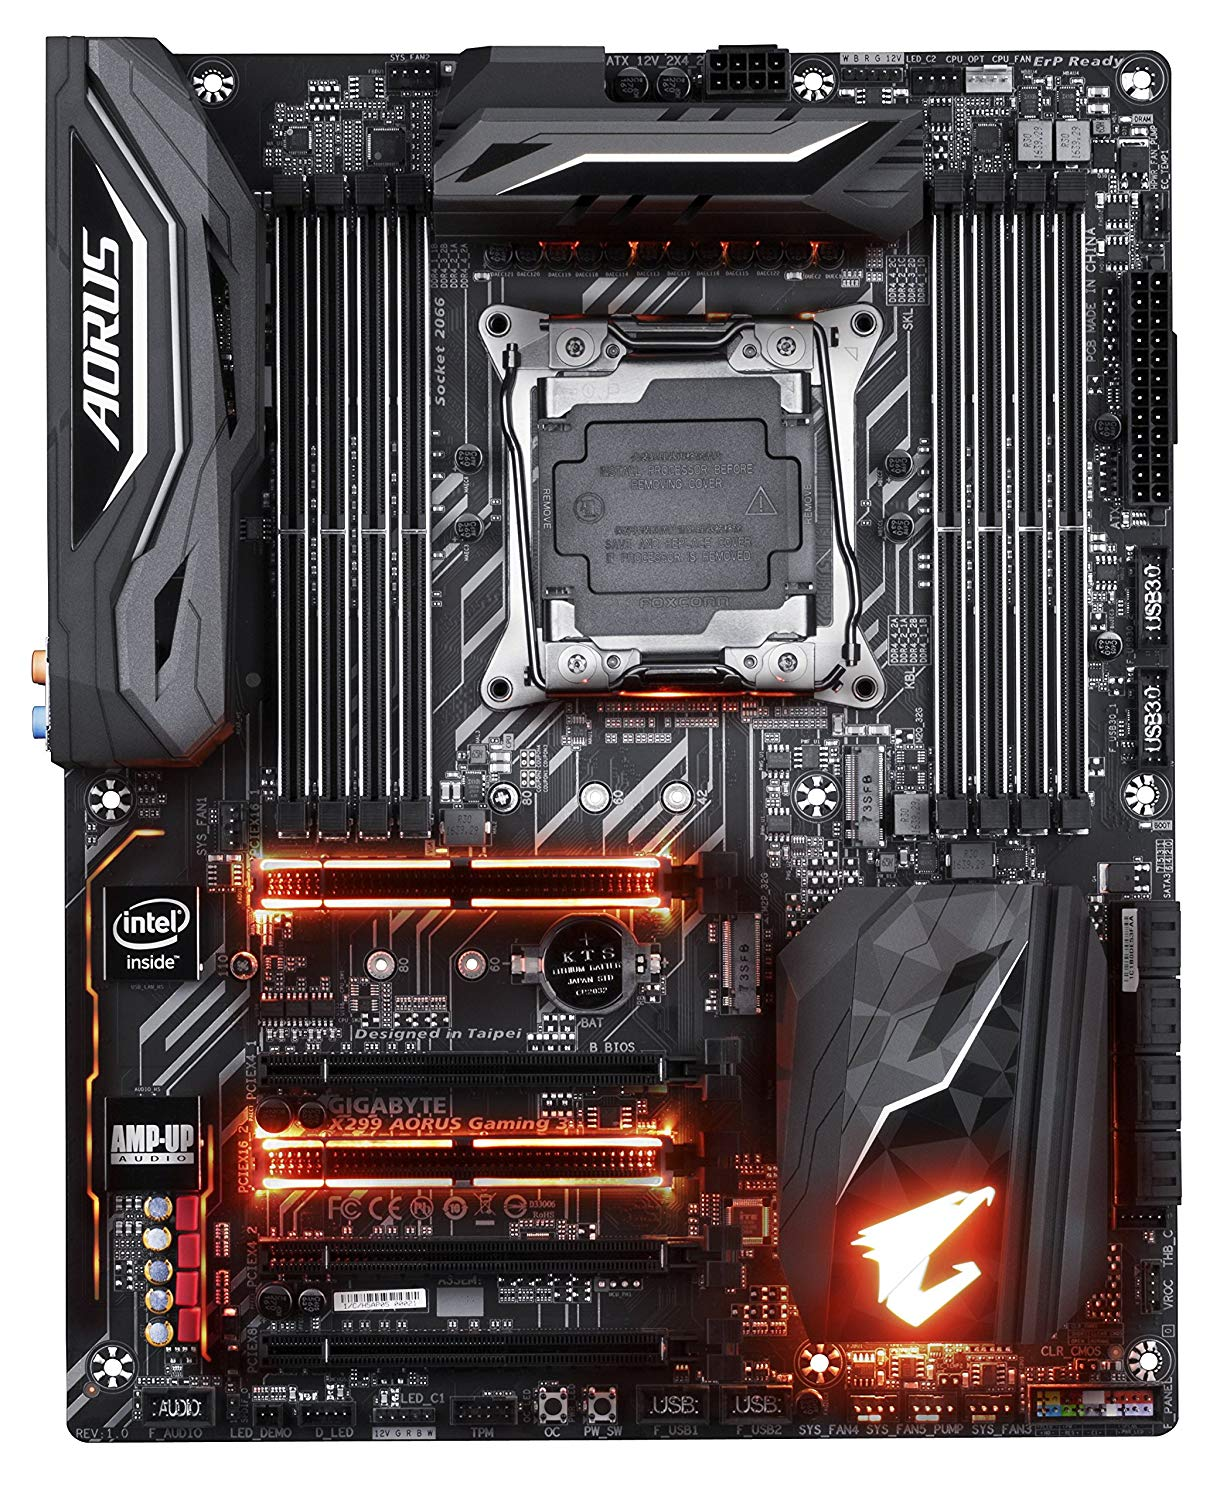
\includegraphics[width=195pt]{refs/Gigabyte_AORUS_X299.jpg}
	\end{frame}


\section{CUDA API}

\begin{frame}
\frametitle{Applications}
	\centering
	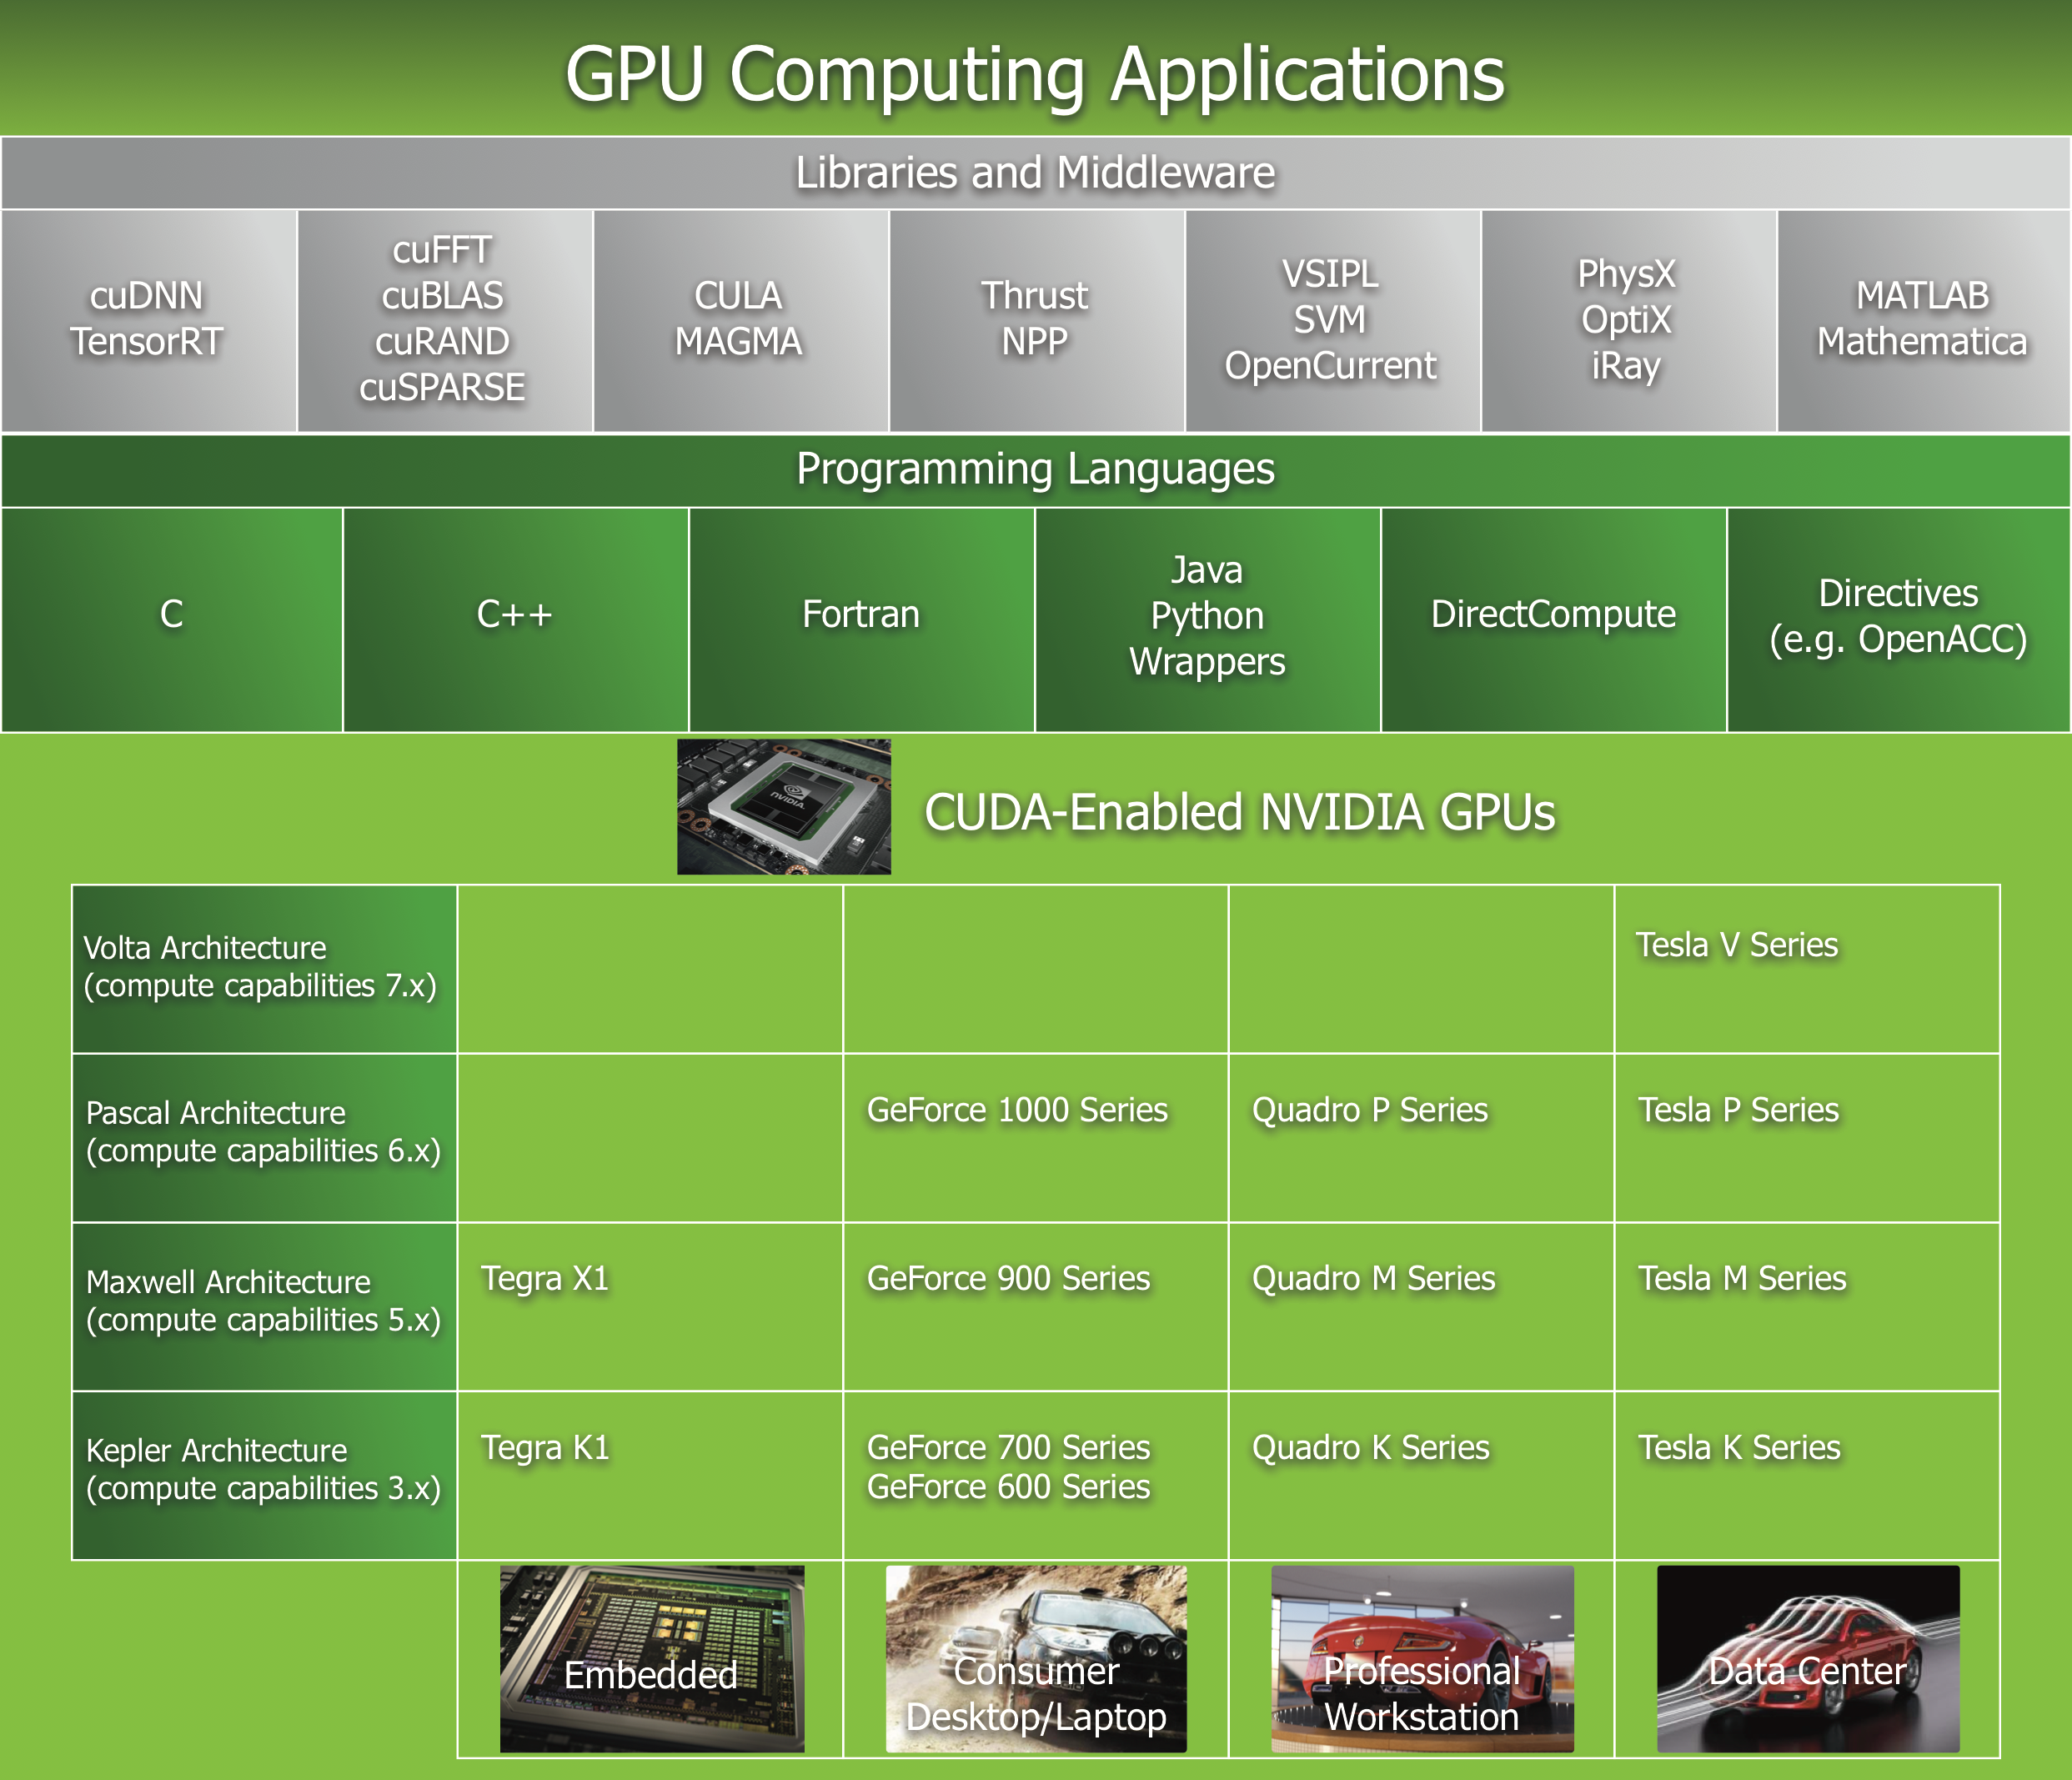
\includegraphics[scale=0.09]{refs/cuda_application.png}
	\\ more \href{https://developer.nvidia.com/language-solutions}{language solution}
\end{frame}

\begin{frame}
\frametitle{PyCUDA}
	PyCUDA lets you access Nvidia's CUDA parallel computation API from Python.
	\begin{itemize}
		\item Maps all of CUDA into Python.
		\item Enables run-time code generation (RTCG) for flexible, fast, automatically tuned codes.
		\item Added robustness: automatic management of object lifetimes, automatic error checking
		\item Added convenience: comes with ready-made on-GPU linear algebra, reduction, scan. Add-on packages for FFT and LAPACK available.
		\item Fast. Near-zero wrapping overhead.
		Complete, helpful documentation.
	\end{itemize}
\end{frame}

\begin{frame}
\frametitle{Types of Quantum Processor}
	\begin{block}{\textbf{Silicon Spin Qubits}}
		Electrons or nuclear spins on a solid subtract
	\end{block}
	\begin{block}{\textbf{Superconducting Circuits}}
		currents superposition around superconductor
	\end{block}
	\begin{block}{\textbf{Ion's Trap}}
		Trap ions in electric fields
	\end{block}
	\begin{block}{\textbf{Photonic Circuits}}
		qubits are photons driven in silicon circuits
	\end{block}
\end{frame}

\end{document}

